\RequirePackage[hyphens]{url}
\documentclass[%
a4paper,
DIV12,
2.5headlines,
bigheadings,
titlepage,
openbib,
%draft
]{scrartcl}
\usepackage{amsfonts}
\usepackage{amsmath}
%\usepackage{lm}
\usepackage{ifxetex}
\usepackage{ifluatex}
\usepackage{eurosym}
\usepackage{listings}
\usepackage{fancyvrb}
\usepackage{longtable}
\usepackage{booktabs}
\usepackage{graphicx}
%\usepackage{mathbb}
\usepackage{grffile}
\usepackage{ulem}
\usepackage{tabularx}
\usepackage[export]{adjustbox}
\usepackage[T1]{fontenc}
\usepackage{listings}
\usepackage{titling}
\usepackage{graphicx}
\usepackage{scrpage2}
\usepackage{float}
\usepackage[colorinlistoftodos,prependcaption,textsize=tiny]{todonotes}
\usepackage[pdftex, colorlinks, linktocpage, linkcolor=black, citecolor=black, urlcolor=black]{hyperref}
\usepackage{atbegshi}% http://ctan.org/pkg/atbegshi
\usepackage{placeins}
\usepackage[ampersand]{easylist}
\usepackage{subcaption}
\usepackage{natbib}
\usepackage{multirow}

\AtBeginDocument{\AtBeginShipoutNext{\AtBeginShipoutDiscard}}
\pagestyle{scrheadings}

%%%
\RequirePackage{type1cm}% CM-Fonts including Math-Fonts in all sizes.
\RequirePackage{color}
\RequirePackage{soul}
\setstcolor{blue}

\newcommand{\bscom}[2]{%
  % #1 Original text.
  % #2 Replacement text.
  \st{#1}{\color{blue}\fontsize{8}{8}\selectfont\,#2}}

\begin{document}
%%%

\pretitle{%
  \begin{center}
  \LARGE
  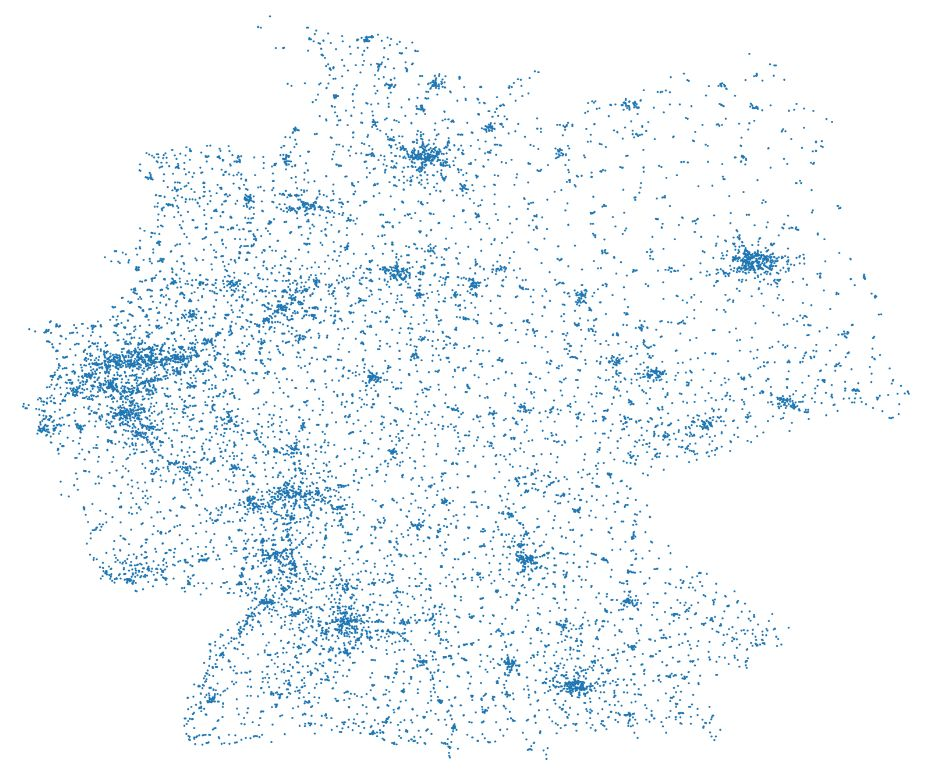
\includegraphics[width=8.5cm,height=8.5cm]{img/all_gas_stations.jpg}\\[\bigskipamount]
	
}
\posttitle{\end{center}}

\providecommand{\tightlist}{%
  \setlength{\itemsep}{0pt}\setlength{\parskip}{0pt}}

\DeclareRobustCommand{\desiredTitle}{
  Intellitank - Prediction of Gas Prices and Route Optimization \\\normalsize{Solution for the informatiCup 2018}
}

\DeclareRobustCommand{\desiredAuthor}{
  \\\\Freya Behrens\\\texttt{freya.behrens@student.hpi.de}\\Hasso Plattner Institute \and \\\\Sebastian Bischoff\\\texttt{sebastian.bischoff@student.hpi.de}\\Hasso Plattner Institute \and \\\\Willi Gierke\\\texttt{willi.gierke@student.hpi.de}\\Hasso Plattner Institute\\\\\\\\\\\\
}

\begin{titlepage}
\begin{center}
   \title{\desiredTitle}
   \author{\desiredAuthor}
   \date{Potsdam, January 2018}
   \maketitle
\end{center}
\end{titlepage}

\pagebreak

\tableofcontents
\pagebreak

\section{Challenge Description}\label{challenge-description}
This year's informatiCup challenge was to predict gas prices of German gas stations up to one month into the future.
Given a route that visits various gas stations consecutively at certain points in time, these gas price predictions should be taken into account to calculate the most efficient fueling strategy.
Given a car's maximum fuel capacity and its average consumption, this strategy determines how much gas one should fill up at each gas station such that the expenses for gas to traverse the route are minimal.

In our solution, we focused on the data prediction task and explored both traditional additive models for time series prediction and explored more modern approaches which use neural networks.
In this process we leveraged some external information like holidays and considered the spatial features of the gas stations.
In addition, we deployed a web application that displays the best filling strategy based on our predictions given user-defined routes within Germany.

This work is structured as follows.
First, Section \ref{data-exploration} gives an overview over the provided data as well as related studies.
Secondly, Section \ref{prediction-model} describes models we applied, how we preprocessed the data, how the models were trained and validated.
Section \ref{fixed_path_gas_station_problem} outlines how the optimal filing strategy can be computed.
In Section \ref{implemented-application} we characterize the application we built using the collected knowledge from the previous sections.
In Section \ref{future-work} examines how to extend and improve the used approach further.
Finally, in Section \ref{appendix} supplementary Figures are provided.

\section{Data Exploration and Feature Engineering}\label{data-exploration}

\textbf{Overview} The given dataset consists of 15226 different gas stations in Germany.
14961 of them reported their gas prices in the period from 2013 to 2017.
The unit of the given prices is deci-cent.
Additionally, the coordinates, addresses and owning companies are available.

\textbf{Existing studies}
%\bscom{}{Existing anlysis on gas station data is available. Studie: \url{www.rwi-essen.de/presse/mitteilung/164/} - similarities and differences to our findings}
%\bscom{}{TODO: Willi: ADAC zum thema.... Gas station prices are of interest to a lot of people, several apps to predict, bunderkartell amt interessant -> information already available} \\
The ADAC (General German Automobile Club) conducted a study between October 2013 and September 2014 which monitored the gas prices of over 14.000 German gas stations\footnote{\url{https://www.adac.de/infotestrat/adac-im-einsatz/motorwelt/jahressprit.aspx}}.
They found out that the prices highly correlate with the time of the day.
Specifically, the gas prices are at a maximum between 10 p.m. and 5 a.m.
During the day, the prices slowly decrease until they reach a minimum between 6 and 8 p.m.
Overall, the gas prices change by 8.7 cent per day on average.
The same patterns where found by multiple studies of the RWI Essen.\footnote{\url{http://www.rwi-essen.de/presse/mitteilung/164/}}~\footnote{\url{http://www.rwi-essen.de/presse/mitteilung/212/}}
The most recent study was conducted based on gas prices of nearly all German gas stations between March and April 2016\footnote{\url{http://www.rwi-essen.de/presse/mitteilung/239/}}.

\textbf{Price Change Dynamics} \begin{figure}
  \centering
    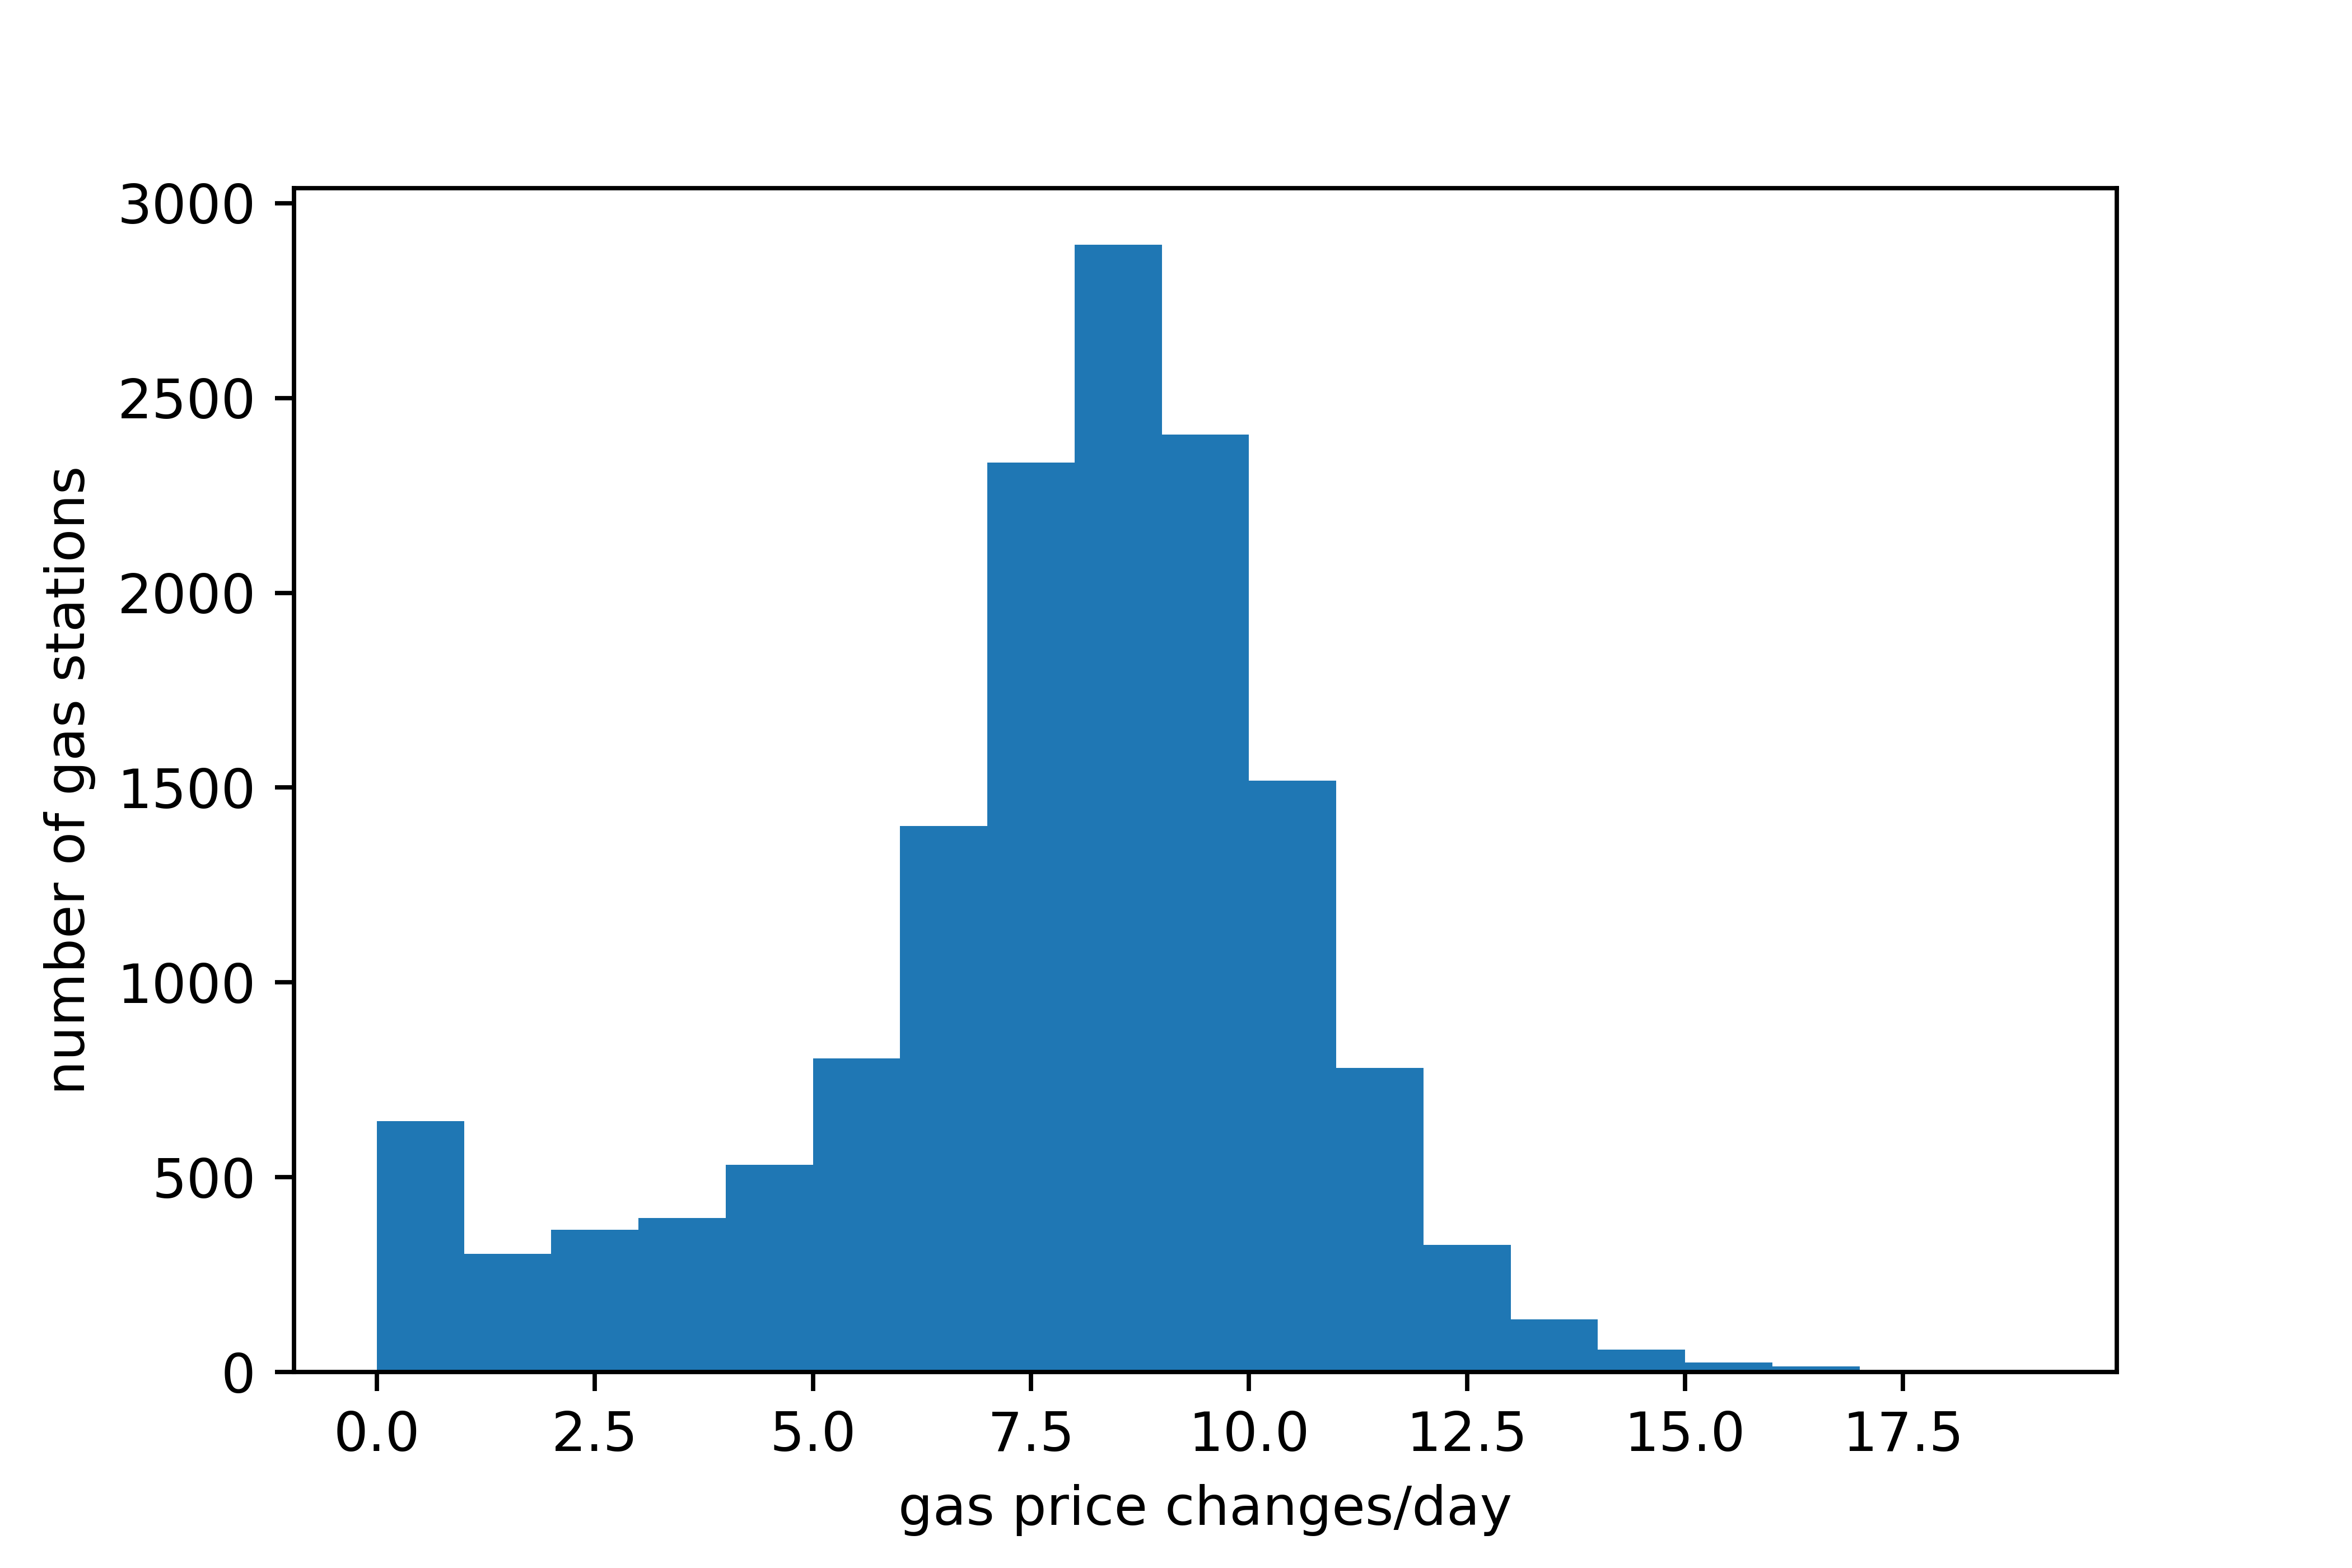
\includegraphics[width=0.7\textwidth
    ]{img/gas-price-change-rate.png}
    \caption{Histogram of average gas price changes per day for all gas stations with bin width 1. We excluded outliers which have a higher change rate than 17 changes per day for visualization purposes.}
    \label{fig:gas-price-change-rate}
\end{figure}
Gas stations do not change their prices at predetermined points in time but react dynamically to the daily situation.
They can change the existing price to a new one anytime they want, which is why the given data is rather an event series than a time series which has equally spaced intervals between the prices.
Gas price updates are distributed from almost zero up to 40.6 changes per day and station.
645 gas stations change their price less than once per day.
The most dynamic gas station changes its gas price approximately 40.6 times per day.
The average gas station changes its price 7.8 times per day with a standard deviation of 2.9 as one can see in Figure \ref{fig:gas-price-change-rate}.
% Also, some stations close down during the night.
Since event series are difficult to compare to one another due to the irregular updates, we experimented with different resolutions of time series derived from the event series.
These reached from one minute to an hour.

\begin{figure}
\vspace{-10pt}
  \centering
    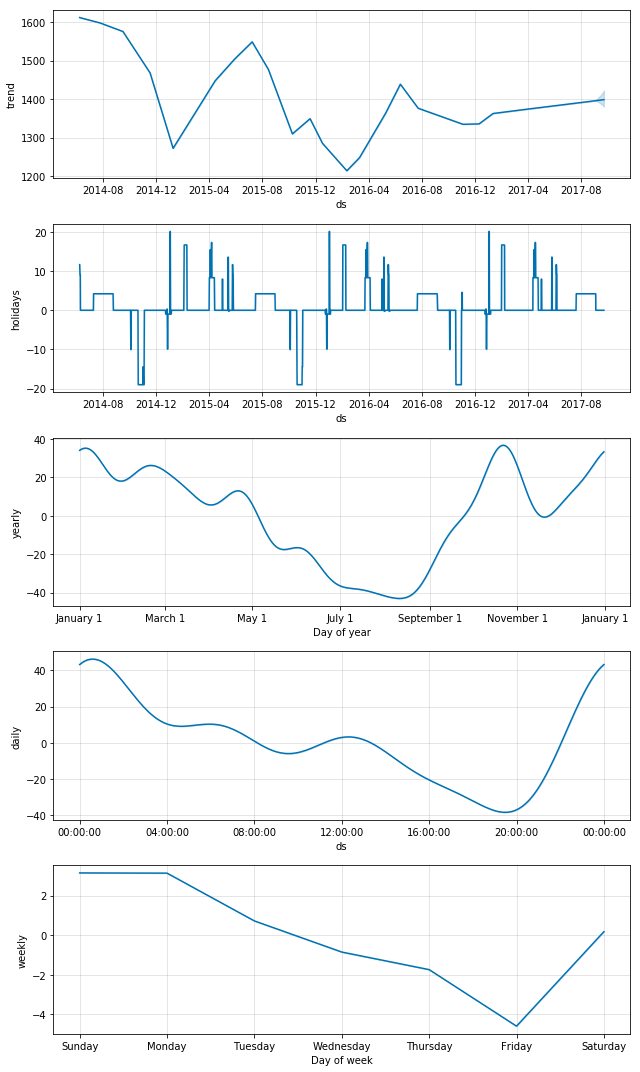
\includegraphics[width=0.85\textwidth
    ]{img/prophet-model-1905.png}
    \caption{Decomposition of different factors for the additive model learned on the data of gas station \textit{1905}. The unit of the y-axes is deci-cent.
    %\bscom{}{Look on individual holidays with $m.plot_forecast_component(forecast, 'superbowl')$}
    }
    \label{prophet-factors}
\end{figure}
\begin{figure}
  \centering
    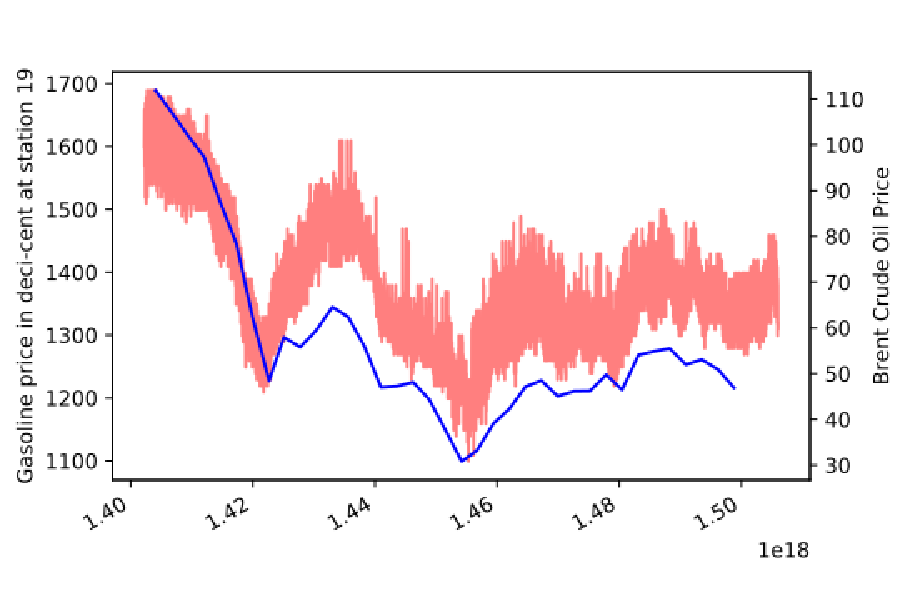
\includegraphics[width=0.7\textwidth
    ]{img/comparison-gas-and-oil-price.pdf}
    \caption{Gas price at gas station 19 in comparison with the Brent Crude Oil Price.}
    \label{comparison-gas-and-oil-price}
\end{figure}

\textbf{World market crude oil price}
The plot of the \textit{trend} in Figure \ref{prophet-factors} shows a high correlation with the oil price as can be seen in Figure \ref{comparison-gas-and-oil-price} during the time of available data.
%Calculate correlation between gas price and different crude oil and gas markets (gas price as average/median over all German gas stations or average correlation over all gas stations)\\
One can see a strong correlation between different gas and Crude Oil markets and the gas price at the gas stations. 
We picked randomly gas station \textit{19} as an example gas station and the Brent Crude Oil Price, which have a Pearson's correlation coefficient of \textit{0.83} and an overall similar development as one can see in Figure \ref{comparison-gas-and-oil-price}.
%\bscom{}{What is the meaning of this, do we include this in our model, is there a lagged correlation? => How fast to the gas stations react to a changing crude oil price?} \\

\textbf{Geo-location} To understand how gas stations are influenced by the position they are located in, we explored Berlin as an example in Figure \ref{fig:berlin-map}.
From the distribution of slightly cheaper gas stations in some areas (e.g. eastern part of Berlin) we can deduce that the structural position of the gas station has an impact since a clustering can be observed.
\begin{figure}
  \centering
    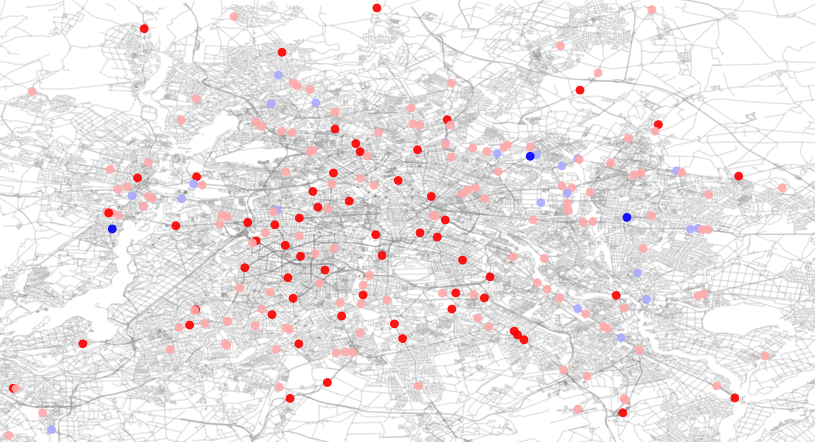
\includegraphics[width=0.8\textwidth
    ]{img/berlin_avg_gas_station_price.png}
     \caption{Average gas prices in Berlin of all time in dataset (\textit{grey}: streets, \textit{red}: more expansive gas stations, \textit{blue}: cheaper gas stations)}
     \label{fig:berlin-map}
\end{figure}
Also, gas stations close to highways are usually more expensive as can be seen in Figure \ref{fig:all-germany-avg}.
In addition, we hypothesized
that the neighboring gas stations have an impact on each other because of their direct competition.
We evaluated whether an understanding of the local dynamics could be learned and benefit by the neural nets.

\textbf{Additional Features} 
Different features which are not provided in the original data can be included for the prediction like distance to the next Autobahn, the street size where the gas station is located and other topological properties.
Dynamic features like traffic information, traffic density, temperature, weather etc. can not directly be incorporated.
If they should be part of the model, one has to predict them as well because we do not know their value in the time period we want to predict.

\section{Prediction Model}\label{prediction-model}
We developed two kind of prediction models. 
One is based on additive models incorporating non-linear trend and the other on recurrent neural networks.
The first model was chosen as a baseline to compare with and because of their easy train-ability and deploy-ability in a live environment.
The advanced model incorporates special aspects of periodicity, like holidays and yearly aspects.
Neural networks are well known for their capability to model very complex functions and especially recurrent networks are popular for time-dependent prediction tasks.
Their major drawback is the costly training and deployment.
This is the reason why we only experimented with different neural network architectures to show how special aspects of the gas prediction task benefit from this sort of model.
Building on these findings it is most probably possible to build an even more powerful architecture.

\subsection{Additive Models}\label{additive-models}
\textbf{Model}
We chose to use the additive model \textit{Prophet} which was developed and open-sourced by Facebook\citep{taylor2017forecasting}.
It was optimized for predicting observations that follow human-scale seasonalities meaning that the data should highly depend on the day of the week or time of the year.
It also features built-in support for holidays which was a major key since previous studies already found out that gas prices and holidays are closely connected.
The core of \textit{Prophet} is an additive regression model.
It consists of four main components.
The first one models the global trend using a linear or logistic growth curve.
It can automatically detect trend changes by selecting changepoints from the data.
Two components detect yearly seasonalities using Fourier series and weekly seasonalities using dummy variables, respectively.
The fourth component is a list of holidays that can be provided by the user.
During the training process, these components are fitted to the data such that their individual predictions for the forecast can simply be ensembled.

\textbf{Insights}
To understand the seasonality of the gas prices and how holidays affect them, we trained \textit{Prophet} on the data. 
In the following, we explore the learned components of the model that contain the trend, impact of holidays and seasonality.
Figure \ref{prophet-factors} shows these different characteristics of the data through the learned model on gas station \textit{1905}.
To train the model on the historical prices of a gas station, it needs approximately 1.5 minutes.
The persisted model is smaller than 600KB.
Thus, \textit{Prophet} provides a lot advantages over neural networks which need 20MB for the weights for one gas station and train a lot longer.
This becomes even clearer when one recalls that we need to train one model for each of the 15000 gas stations.

\textbf{Periodicity and Holidays} 
Considering the \textit{holidays} subplot of Figure \ref{prophet-factors} one can see the impacts of various holidays on the gas price suggested by the model.
\begin{figure}
\begin{subtable}{0.5\textwidth}
\centering
\begin{tabular}{c|c|c}

Holiday Name    & Date   & Price Increase            \\ \hline
New Year's Day  & 01.01. & 2.1 ct                       \\ \hline
Ascension Day   & 14.05. & 1.5 ct                      \\ \hline
Winter Holidays & 02.02. & 1.4 ct                      \\ \hline
Whit Sunday     & 08.06. & 1.1 ct                      \\ \hline
Easter Monday   & 06.04. & 0.9 ct                      \\ \hline
Whit Monday     & 09.06. & 0.9 ct                      \\ \hline
May Day         & 01.05. & 0.9 ct                      \\ \hline
Easter holidays & 01.04. & 0.7 ct                      \\ \hline
Good Friday     & 03.04. & 0.7 ct                      \\ \hline
Easter Sunday   & 05.04. & 0.5 ct                      \\
\end{tabular}
\caption{Maximal price increases for certain holidays}
\label{maximal-price-increases}
\end{subtable}
\begin{subtable}{0.5\textwidth}
\centering
\begin{tabular}{c|c|c}
Holiday Name    & Date   & Price Decrease                   \\ \hline
Autumn Holidays     & 20.10.       & 1.7 ct                      \\ \hline
Day of German Unity & 03.10.       & 0.9 ct                      \\ \hline
%Day of & 03.10.       & 0.9                       \\
%German Unity &        &                        \\ \hline
Boxing Day          & 26.12.       & 0.8 ct                      \\ \hline
Summer Holidays     & 10.07.       & 0.2 ct                      \\
\end{tabular}
\caption{Maximal price decreases for certain holidays}
\label{maximal-price-decreases}
\end{subtable}
\caption{Effects of the different holidays on the gas price. The dates of the holidays are exemplary for 2015.}
\end{figure}
When analyzing the influence of the holiday components to the gas price, one can note that during most holidays the prices increase while there are also a few holidays that lead to a decreased price on average.
The holidays that contribute to increased prices can be found in Figure \ref{maximal-price-increases}.
Note that the prices are especially increased during the Easter holidays in April.
This finding is covered by the numerous studies that have been conducted by the ADAC in the past\footnote{\url{https://www.adac.de/infotestrat/adac-im-einsatz/motorwelt/benzinpreis\_drama.aspx}}.
In turn, holidays that lead to decreased prices on average can be found in Figure \ref{maximal-price-decreases}.
Our hypothesis is that customers tend to stay at home at the specified holidays which leads to a reduced demand for gas resulting in lower prices.

\textbf{Daily and Weekly Seasonality} 
We would furthermore like to draw the attention particularly to the components that model the daily behavior of gas prices.
According to the learned properties, the gas prices are the lowest between 6 p.m. and 8 p.m. and raise afterwards to a daily high between 10 a.m. and 4 a.m.
These findings coincide with those of the ADAC and the RWI Essen that we presented earlier.
While the model learned that the gas prices change by up to eight cent per day, the price differences at fixed times between various days of the week only vary by up to 0.6 cent.
At a first glance, this might look counter-intuitive.
However, this finding is covered by observations of the newspaper \textit{Die Welt}\footnote{\url{https://www.welt.de/wirtschaft/energie/article138897786/Zu-welcher-Uhrzeit-man-am-billigsten-tankt.html}}.


\subsection{Neural Networks}
Our models differ in the number of gas station's time series they take as input, their output and the internal architecture.
All of them share the recurrent connection between states as the principal architecture which is a characterization recurrent neural networks.
In many recent publications convolutional neural network are used for problems previously only solved by recurrent neural networks because convolutional neural network are not that much affected by the vanishing gradient problem and are easier to train.
Nonetheless we used recurrent neural networks because they are designed for data with a time component and seemed for us the natural choice.
As future work one could implement convolutional neural networks as well.
We implemented and evaluated our models with \textit{tensorflow}\citep{abadi2016tensorflow}.

\begin{figure}
  %\centering
  	\begin{subfigure}{0.45\textwidth}
    \begin{center}
    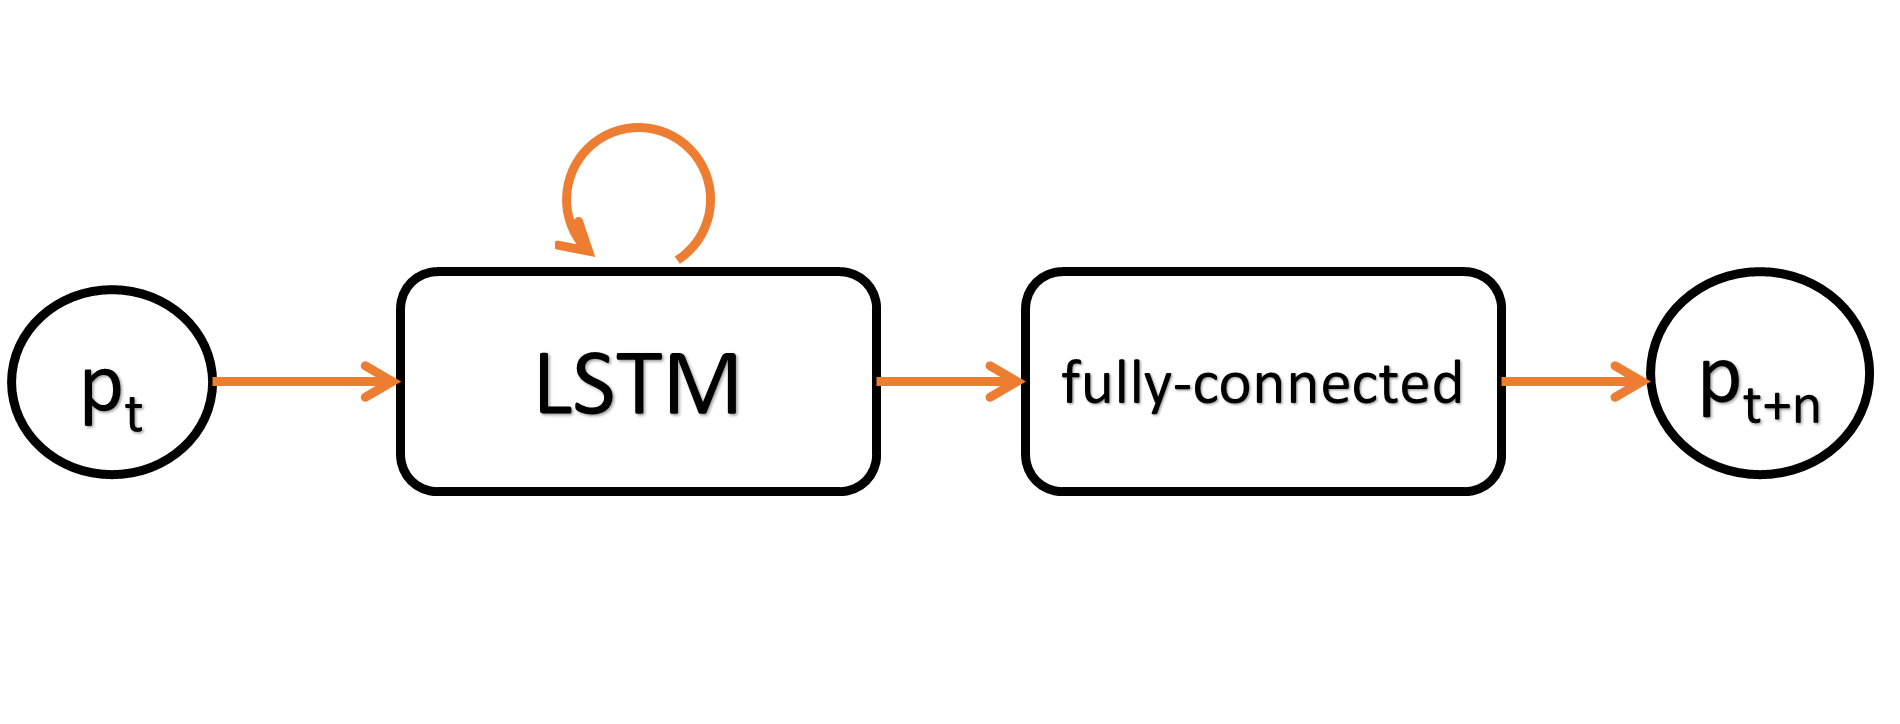
\includegraphics[width=1\textwidth]{img/simple-model.png}
    \end{center}
     \caption{\textbf{Simple model} with the price at the time step \textit{t} as input, and the predicted price at the $n^{th}$ next time step as output}
     \label{simple-model}
  	\end{subfigure}
    \begin{subfigure}{0.45\textwidth}
    \begin{center}
    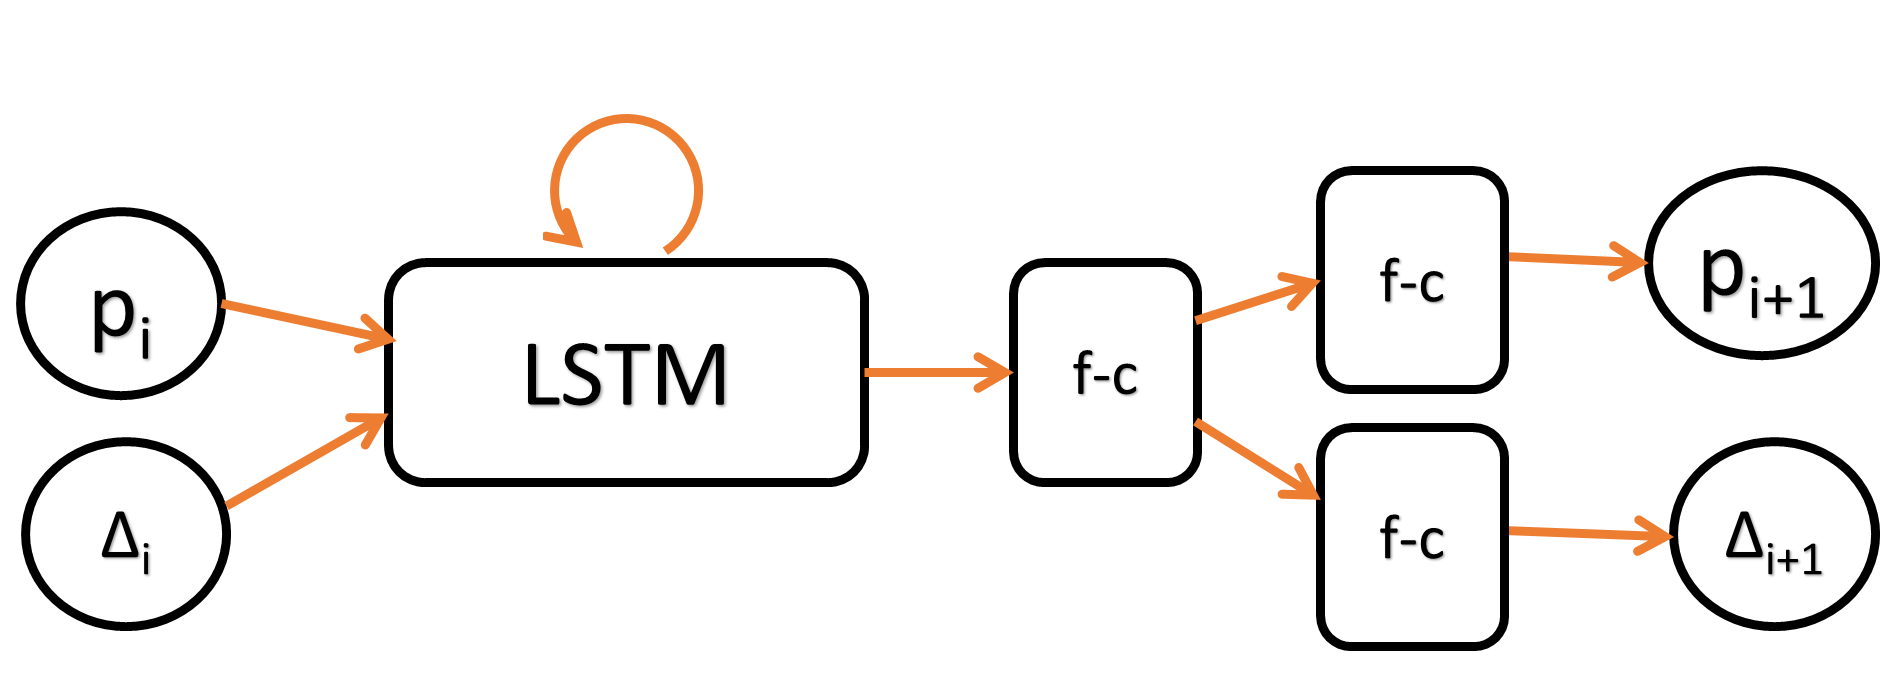
\includegraphics[width=1\textwidth]{img/change-model.png}
    \end{center}
     \caption{\textbf{Change point model} with the price change event as input and the predicted next event as output (both made up of the price update $p_i$ and the time $\delta$ to the last event)}
     \label{change-model}
  	\end{subfigure}
    \caption{The two neural neural network architectures we used to predict the gas price}
\end{figure}

\textbf{Simple Model} The first model receives a fixed-length time series with equal distances between the records of a gas station as input and can predict the future price.
The length of the time series is configurable and depends on the task one wants to solve.
The length and the rate of resampling of the original time series, which yields the equidistant input, greatly influences the amount of training data the preprocessing produces.
The model either predicts just the price for the next time step or, when trained on corresponding data, prices arbitrarily into the future.
We constrained the input data to fixed-length to mitigate the vanishing gradient problem in recurrent neural networks but we could also learn on variable-sized inputs.
We are using a long short-term memory layer followed by a fully connected layer which predicts the price for the next time step as depicted in Figure \ref{simple-model}.

\textbf{Change Point Model} The second model has a fixed-length event series as input, where the records are not equidistant and not each event series might cover the same time span.
The input and output are events consisting of the gas price and the time since the last change as proposed by \citet{du2016recurrent}.
This has the advantage over the first model that the model does not have to learn the significance of the change points based on the resampled and therefore masked input.
This input representation expresses more clearly that there are specific points in time where the price is changing abruptly. 
The network is forced to learn the correct time interval instead of having the possibility to just estimate it roughly as in the first model where the cost function over the resampled time series does not penalize errors that hard.
To learn this more complex problem the model consists of a long short-term memory layer, followed by a fully-connected layer and from there branching two fully-connected layer as in \ref{change-model}. One is predicting the next gas price and the other the time until this gas price change.

\textbf{Additional Gas Stations} The additive models in Section \ref{additive-models} as well as the two neural network models described in this section only use the time series of one gas station as input and therefore can not learn the interactions between multiple gas stations.
In the case of the neural networks this can be easily extended by adding the time series of additional gas stations as input and add them as outputs which should be predicted.
This is necessary because when the network is predicting the future, it needs the additional gas stations also as input to predict the next time step.

\textbf{Extensions} One possible extension could be to predict the development of all gas stations in parallel.
This would result in a network which gets the time series of all gas stations as input and predicts the price development of all gas stations.
With this information the network would be able to learn complex interactions between all stations.
The extension could be further enhanced by including static features of each gas stations like the distance to the next Autobahn, Bundesstra{\ss}e, Autobahn junctions or the area they are located in (business parks, industrial parks, residential areas etc.).
We implemented this features with the \textit{Overpass API} of \textit{OpenStreetMap} but did not have the computing power to train such a big model.
The static features would enable the network to find clusters of similar behaving gas stations and could consider them separately.

\textbf{Experiments}
To check the hypothesis from Section \ref{data-exploration}, that subsets of the gas stations e.g. close gas stations have an influence on each other, we performed some tests without statistical significance.
We studied this by adding additional gas stations to the input data but did not have the necessary computing resources to calculate this for all gas stations and therefore we can not make universal statements.
The data is split into 60\% training data set, 10\% validation data set and 30\% test data set with each data set extracted from the corresponding part of the time series.

We randomly picked the gas station \textit{15205} in Sonthofen as the gas station we want to predict the prices for.
When we fed in the gas stations \textit{15204}, \textit{15206}, \textit{15209} and \textit{15210} which are also located in Sonthofen as additional gas stations into the network, we achieved a minimal mean squared error of circa 51 on the test set at the point of the training process where the validation set error is minimal.

The same procedure for the four randomly picked gas stations \textit{3920}, \textit{9941}, \textit{6226} and \textit{9304} yields a mean squared error of circa 84.
This result shows that the neural network can better predict the development of the gas price at one gas station if it has the data for nearby gas stations.
This indicates that the model can account for local developments such as the race for the lowest gas price in the city between the gas station operators and therefore the most customers.

In another experiment we fed in the gas stations \textit{6249}, \textit{1270}, \textit{734} and \textit{8964} as additional ones which are located in different federal states but all have \textit{Aral} as owning company. %like the station we want to predict the gas prices for.
With this additional gas stations we achieved a mean squared error of circa 29 which indicates a strong connection between the gas stations of one owning company in this case \textit{Aral} which is stronger than the connection to nearby gas stations.

\subsection{Validation of Prediction
Models}\label{validation-of-prediction-models}
\begin{figure}
\vspace{-10pt}
  \centering
    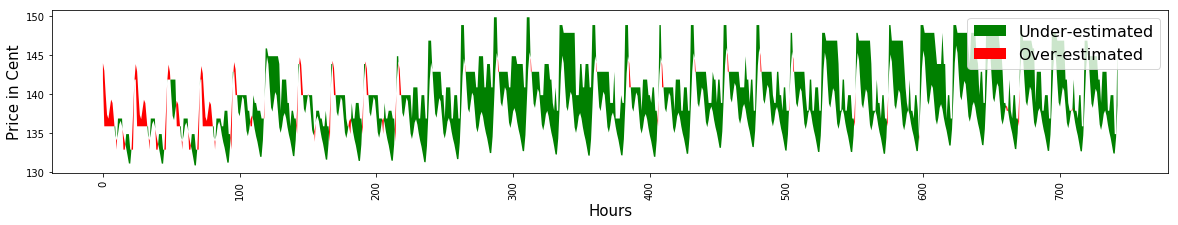
\includegraphics[width=0.85\textwidth
    ]{img/prophet_validation.png}
    \caption{Comparison between the predicted last month of the prices of gas station \textit{1920} and its ground truth. The colored area represents the error. Green means the model under-estimated the price, while red illustrates over-estimation. The mean squared error in this example is 2561.
    }
    \label{prophet-validation}
\end{figure}
\textbf{Evaluation of Prophet} To validate the additive model, we randomly sampled gas stations, fitted the model on the historical prices while leaving out the last month.
We then predicted the last month using the model and calculated the mean squared error between the predicted prices and the ground truth of circa 3425.
In Figure \ref{prophet-validation} one can find the comparison between the prediction and the ground truth for the random station \textit{1920}.
The prediction was performed for every hour in the time frame starting at the 21st of August to the 21st of September.
Note how the model started under-estimating the price once the summer holidays ended after the first third of the time frame.
This shows how dependent the model on specified holidays and vacations is.\\

\textbf{Evaluation of the neural networks}
Because of lack of computation sources, the models we implemented only used the two last days preceding a prediction sampled at a 15 min rate as training data.
As a consequence, these models are less likely to learn seasonality or special reoccurring events such as the start of holidays, since they have to discover within only two days, that such an event is occurring.
Because the underlying event series is difficult to evaluate, the cost function we are fitting for the example gas stations is the mean squared error.

When we optimize on the mean squared error, the duration of how long a price is displayed at the station plays a role. 
It is more beneficial for a model optimized on mean squared error to be precise at a price that is has a long duration.
Small changes are less relevant for this model.
This drawback is considered by the event based neural network.
Since it is optimized on the mean squared error on every event, every change is weighted the same within the loss function.
This is why we would expect the precision of the event model to  have an competitive advantage, where small changes occur.
Routes occurring in times where these changes are frequent, could benefit from this approach.

\textbf{Interesting Test Routes} Since the implementation uses the additive model, we will focus our example routes on where we believe our model will perform especially well or bad.
The big advantage of the model is the use of external information like holidays.
We expect this advantage to be visible in the time shifted 'Bertas Route' to 11.05.2016 (a common day), 26.08.2016 (Summer holiday Baden-Wuertemberg), 8.1.2016 (winter holiday Hessen). 
Also, because our model captures weekly periodicity well, we expect it to handle the prediction in September - Oktober 2017 good as well and have prepared a route from Potsdam to Berlin.

\textbf{Summary}
What we have seen during our data exploration and model fitting processes is, that the underlying structure of price change behavior is very periodic.
This explains, that the models could be useful for a week of price prediction, when the underlying trend of the crude oil price is known.
Unfortunately, a model for the prediction of the crude oil price is very difficult, because its fluctuation are mostly dependent on the political and economical context events\footnote{\url{www.forbes.com/sites/michaellynch/2014/12/15/predicting-the-oil-price-smart-vs-lucky}}.
Ideally, these relevant events could be detected and extracted in a real-time event database like \textit{GDELT}\footnote{\url{www.gdeltproject.org}} and adaptively influence the predictions.

\section{A Filling Strategy for the Fixed Path Gas Station Problem}
\label{fixed_path_gas_station_problem}

\subsection{Optimal Solution with Perfect Knowledge}
\textbf{Problem Statement} In the \textit{Fixed Path Gas Station Problem with Unlimited Refills}, given gas stations $S_i$ with $0 \leq i \leq n$ each with a gas cost $cost_i$, a fixed path $P = (S_0,S_1, ..., S_n)$, a tank capacity $c$ and distances $d_{ij}$ with $0 \leq i \leq j \leq n$ we want to find an optimal filling strategy $f: S \rightarrow R$ so that we can reach $S_n$ with $f$ and $f$ has the least costs.

\textbf{Naive Solution}
In the example of the task description a naive approach was applied to the Berta Benz Memorial Route.
A maximal fullness at each point of the journey can be ensured by filling up the tank at each gas station on the way, if the remaining route is long enough to require it.
This means the solution will always reach the target with the given filling strategy, but might not reach an optimal price.
If at one station $a$ the tank is filled up completely and just shortly afterwards follows a cheaper gas station $b$, the price could have been reduced by filling up only enough at $a$ to get to $b$ and then filling up completely there.


\textbf{Dynamic Programming Approach}
An optimal solution for the problem can be found in $O(n log(n))$.
We will just give an intuition of its workings, for details see \cite{khuller2007fill}. 
All in all, the solution can be found with dynamic programming.
This is possible because the solution of the fixed path problem is a combination of optimally solved subproblems.
Given a path, the subproblems that should be solved are divided at those gas stations that fulfill the property of a so-called \textit{break point} $b$.
A break point marks where the tank must be empty and thus the remaining length of the path is a separate instance of the problem.
All of them have the property that they are preceded by gas stations that were more expensive and within the tank distance.
Consequently at those stations no more fuel than required to reach the break point should be filled up and the break point is reached with an empty tank.
The remaining smaller problems can be solved by filling up for each station enough to reach the next cheapest one in the reachable distance.
The strategies of the subproblems can be append to construct the overall strategy.

\subsection{Real-World Problems and Extensions}
The assumptions of the problem do not map very well to the real world.
Usually a gas stop has an influence both on the duration of a route, but might require detours to reach gas stations off the route. 
Both of them could be introduced as optimization criteria to make the model more realistic.
Additionally, if the route is optimized on predicted values, new properties of the optimization can be considered.

\textbf{Optimizing on Time} 
In order to minimize the duration of a trip a car driver can try to minimize the number of stops at a gas station as well as the price.
Small fluctuations in the price at many gas stations on the route can cause a filling strategy derived by the introduced algorithm which has many stops with only small amounts of refill.
This is why \citet{khuller2007fill} introduce the same problem with a maximum number $\delta$ of filling stops as a constraint and show that this problem can be solved in $O(\delta n^2 log(n))$ time.
When only one gas stop is required on a route, some applications already exist that include the time component.
They optimize on the cheapest and best located gas station and include it in the routing from the start to the destination\footnote{\url{maps.googleblog.com/2015/10/google-maps-making-stressful-times.html} (19.01.2018)}.
Time becomes an even more critical component when the car is electric and can not be refilled in the means of a few minutes. 

\textbf{Optimal Strategies without Perfect Knowledge}
Another difference to the real-world is the uncertainty on the actual gas stations prices in the future.
The predictions derived from any model may not be correct.
If the uncertainty of information is incorporated into an optimization algorithm for the fueling strategy, new problems appear.
Overall, we saw from our data exploration that most gas stations correlate with each other.
If the model learns this, a very far off prediction on one gas station could be mirrored in others that usually correlate with it.
Consequently, a filling strategy containing only highly correlated gas stations would not be very robust towards errors in prediction.
Contrary, filling up at uncorrelated gas stations prevents individual model errors to have a high influence on the overall price of the strategy.
This aspect of a trade-off between risk and optimal outcome in uncertainty is studied in financial mathematics in portfolio creation \citep{markowitz1952portfolio}.
We did not implement any of the proposed strategies, but found them helpful with our reasoning. 

\section{Implementation: Web Application}\label{implemented-application}

\subsection{Functionality}\label{functionality}
\begin{figure}
\centering
  \begin{subfigure}{0.6\textwidth}
	\begin{center}
    
\includegraphics[width=1\textwidth]{img/web_app_screenshot.png}
    \caption{Landing page}
    \label{fig:landing_page}
    \end{center}
  \end{subfigure}
	\begin{subfigure}{0.3\textwidth}
	\begin{center}
    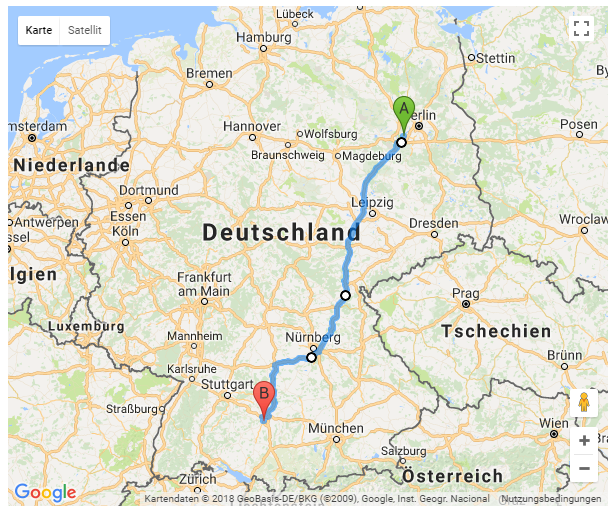
\includegraphics[width=1\textwidth]{img/web_app_route_potsdam_ulm.png}
    \caption{Example Route from Potsdam to Ulm with stops for optimal filling strategy marked}
    \label{fig:example_route}
    \end{center}
  \end{subfigure}
  \caption{Screen shots of our implemented web app. Accessible at \url{http://tofill.dyndns.info:7080}.}
\end{figure}

% Overview
We build a platform which is deployed in the cloud where a user can enter the details of their planned trip (start and destination city, start date and time, maximal distance of a gas station to the fastest route) and information about their car (tank size, current fill level, expected average speed) as can be seen in Figure \ref{fig:landing_page}.
Based on the information from the user our system calculates the fastest route with an online route planning software and displays the resulting filling strategy to the user.
All necessary tank stops along the way are integrated into the fastest route.
The address of the gas station, the predicted gas price and the fuel required for the calculated strategy are highlighted on the map.
\\ % Pros of Continous development
Being able to continuously update this application allowed us to evaluate the real world implications of our algorithms and prediction models easily.
We did not need to generate manual test routes because we had the possibility to adjust the parameters and thus explore further routes.
For example, in early iterations we found that long routes with very similar prices along it would lead to a high number of stops.
As a consequence, we could tweak the filling strategy algorithm to respond to this case as well.
\\ % Assumptions
While we evaluated several different types of models, we were only able to deploy the additive model.
This means that only this model can be explored.
A very strong assumption we make, that is not clearly visible to the user, is to map nearby gas stations onto the route.
The effect of our simplification is visible in Figure \ref{fig:mapping:mapped} in comparison with Figure \ref{fig:mapping:real}.
While the filling strategy is optimal with regards to this mapped scenario, it could differ from the true optimal route.

\begin{figure}
\begin{subfigure}{0.49\textwidth}
    \begin{center}
    
\includegraphics[width=0.5\textwidth]{img/web_app_assumption_not_mapped.jpg}
    \end{center}
  \caption{Geographic positions of gas stations}
  \label{fig:mapping:real}
\end{subfigure}
\begin{subfigure}{0.49\textwidth}
    \begin{center}
    
\includegraphics[width=0.5\textwidth]{img/web_app_assumption_mapped.jpg}
    \end{center}
  \caption{Positions of gas stations as mapped by our algorithm}
  \label{fig:mapping:mapped}
\end{subfigure}
\centering
\caption{Geographic and mapped positions of gas stations within 1km from the route from Potsdam to Berlin%: Real positions of gas stations in comparison \textit{(left)} to mapped positions \textit{(right)}
}
\label{fig:mapping}
\end{figure}

\subsection{Tooling Choices}\label{tooling-choices}
\textbf{Technologies}
We chose to use \textit{Python}since it is a general purpose programming language which has been designed to be easy to understand.
As already mentioned we used the additive model \textit{Prophet} which has been open-sourced by Facebook.
In order to implement the neural network architecture we used TensorFlow.
To efficiently handle data matrices we used \textit{NumPy}\citep{walt2011numpy} and \textit{pandas}\citep{mckinney2010data}.
The latter library provides a high-level abstraction of the underlying data and supports many convenient data processing techniques.
For geo-spatial data exploration we used \textit{geopandas}\footnote{\url{http://geopandas.org}}.
We furthermore used the machine learning library \textit{scikit-learn}.
To quickly develop insides into the data and test prototypes visually, we used \textit{Jupyter}\footnote{\url{https://jupyter.org}}.
In order to build a service using our learned models we chose to use \textit{Flask}\footnote{\url{http://flask.pocoo.org/}} to implement the server since it is very light-weight.
\textit{JavaScript} was used to implement logic in the front-end.
In order to calculate the fastest route between two points and to show the result on a map, we used the \textit{Google Maps API}\footnote{\url{https://developers.google.com/maps/}}.
Neighboring gas stations close to the computed route were fetched using the \textit{Google Places API}\footnote{\url{https://developers.google.com/places/}}.

\textbf{Development Process}
We hosted the source code on and managed the project using tickets at \textit{GitHub}\footnote{\url{https://github.com}} as it provides a very intuitive user interface and the possibility to add further integrations.
As such we set up automated testing on \textit{CircleCI}\footnote{\url{https://circleci.com/}}.
The advantage of \textit{CircleCI} was that it allowed us to integrate it in our private repository without additional fees.
We developed in an agile manner by respecting the agile manifesto\footnote{\url{http://agilemanifesto.org/}}.
We gave feedback on a regular basis, introduced automated testing to ensure finding flaws very early and valued communication and face-to-face interaction a lot.

\section{Future work}\label{future-work}
\textbf{Problems of Electromobility}
In this work we studied the hidden seasonality and correlation between gas prices and other time-dependent values such as the crude oil prices or holidays.
Since humanity is rapidly moving towards the use of electric powered vehicles, the question arises how our approach could be extended to support electromobility as well.
Unfortunately, from the current point of view it does not look like the approach could be ported easily.
A study\footnote{\url{https://www.lichtblick.de/presse/news/2017/07/10/ladesaeulen-check-deutschland-stromtankstellen-kompliziert-und-oft-teuer/}} in 2017 of the enterprise LichtBlick SE found that the prices between offerers of charging stations highly differ.
Currently, users of electric powered vehicles have to register at charging stations for extra non-recurring fees.
This makes spontaneously fueling at new charging stations during traveling extremely expensive.
Additionally, the tariff plans are greatly nontransparent meaning that vendors for example can also charge text messages that have been sent by them.
In general, the price for fueling highly depends on car's loading speed since stations also charge by the time this process spends.\\

\textbf{Adaptions for Electromobility}
In order to support electromobility as well, one would need to know the exact tariff plans of all charging stations and electricity providers.
Furthermore, the customer would be supposed to specify all registrations he is holding with charging stations and providers.
One would also need to take into account the loading time of the car at a given station.
This can highly vary between the station vendors since most German stations offer 11 kW while the Tesla Supercharger\footnote{\url{https://www.tesla.com/supercharger}} delivers up to 135 kW\footnote{\url{https://www.golem.de/news/elektromobilitaet-allego-stellt-die-ersten-ultra-schnellladesaeulen-auf-1712-131831.html} (22.12.2017)}.
For further convenience of the user, one could try to predict when charging stations are not occupied such that the customer is not supposed to wait possibly for hours before he can actually charge his car.

\bibliographystyle{plainnat}
\bibliography{documentation} 
\newpage
\section{Appendix}\label{appendix}
\subsection{Additional Figures}
\begin{figure}[H]
  \centering
    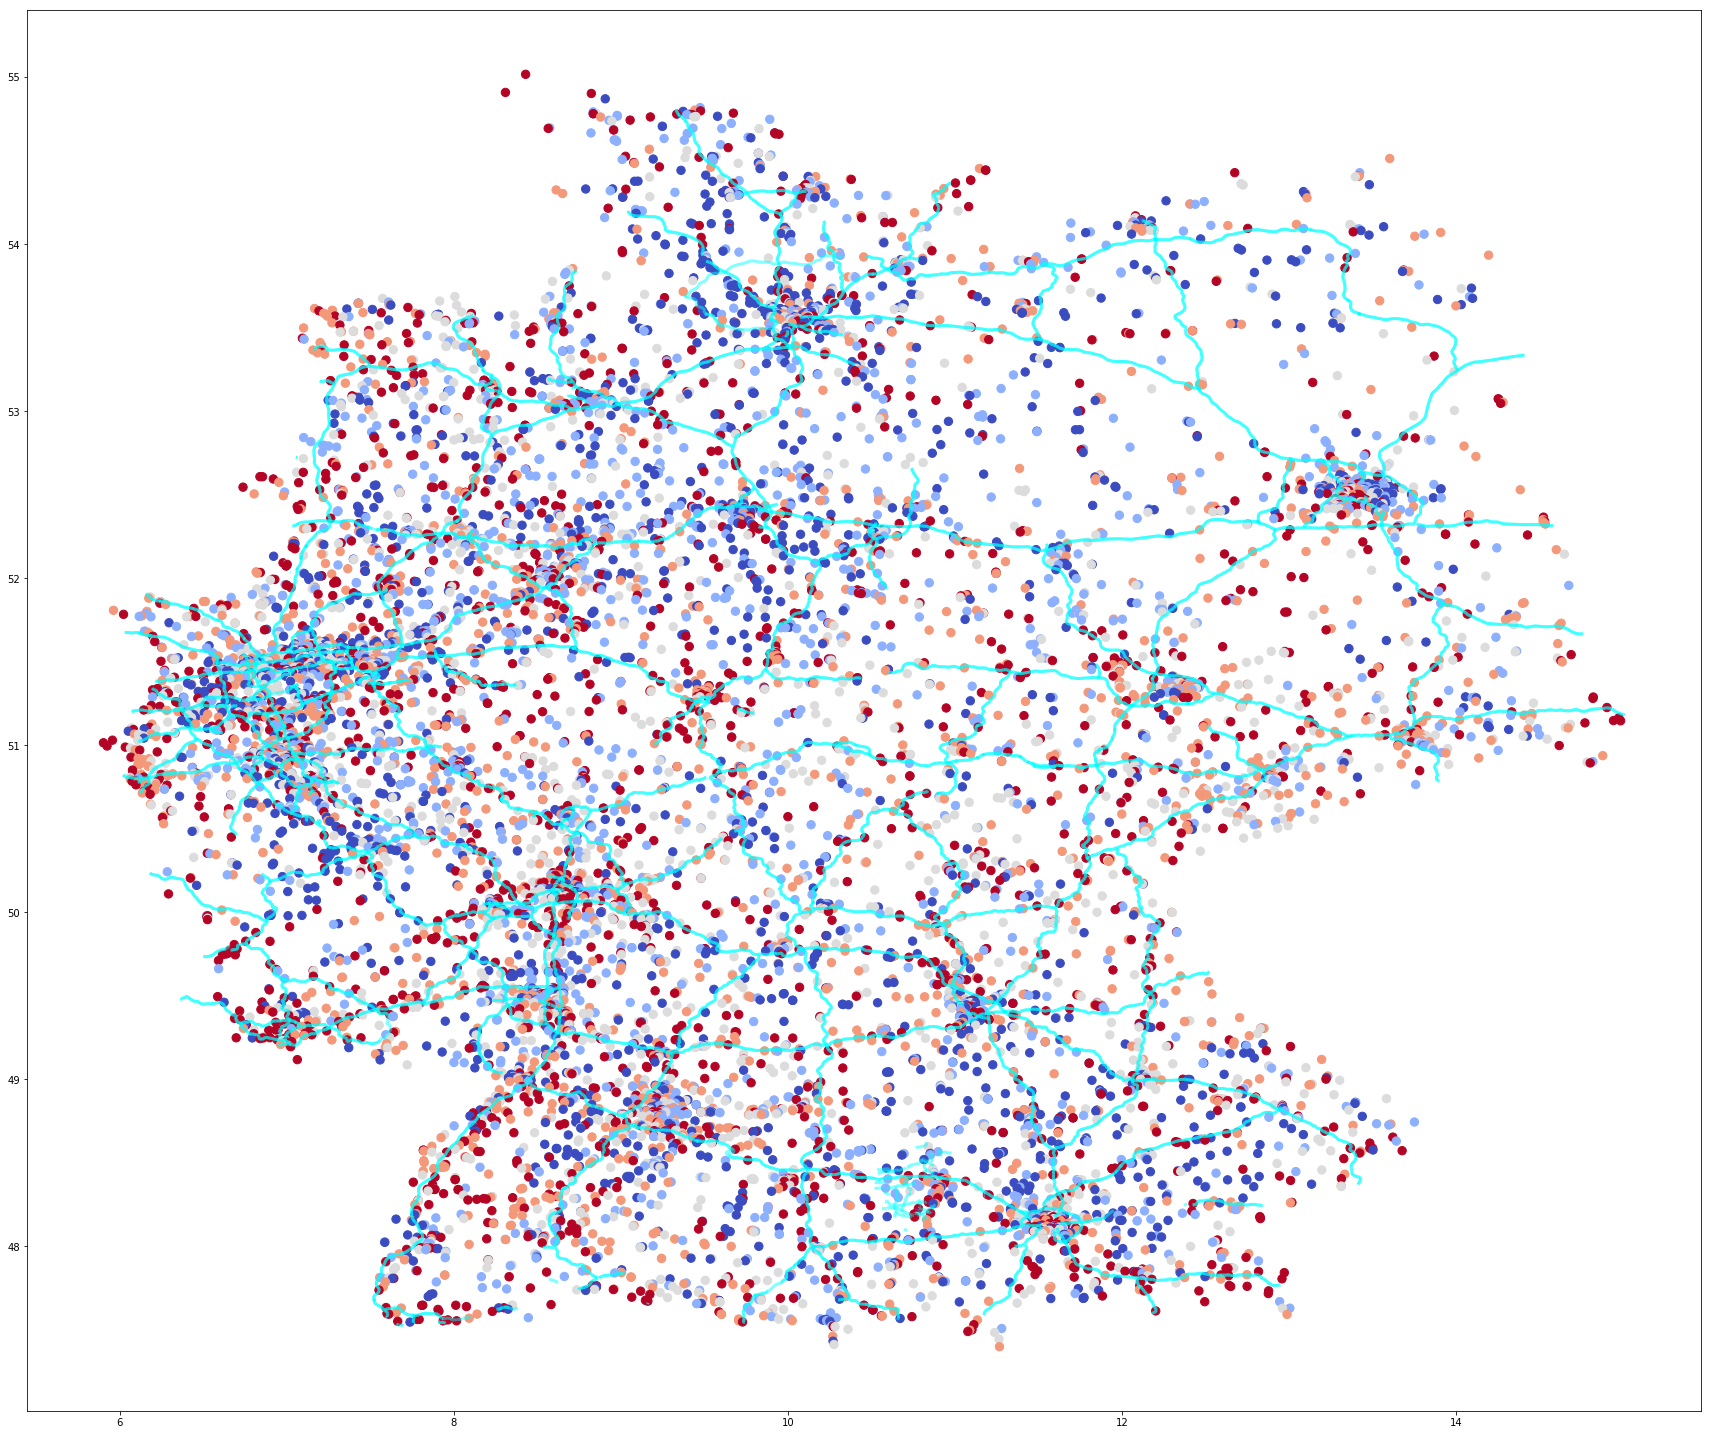
\includegraphics[width=1\textwidth,height=1.05\textwidth,
    ]{img/avg_price_in_all_time.png}
     \caption{Average gas prices in Germany (\textit{cyan}: highways, \textit{red}: more expansive gas stations, \textit{blue}: cheaper gas stations)}
     \label{fig:all-germany-avg}
\end{figure}
%\begin{table}[]
\centering
\begin{tabular}{|l|c|}
\hline
Route & Challenges & Expected Relative Performance \\ \hline
Bertas Route: \\Any day \\(11.05.2016)                  & $\sim$                        \\ \hline
Bertas Route: \\Summer Holiday BW \\(26.08.2016)                          & ++                            \\ \hline
Bertas Route: \\End of winter holiday\\ (08.01.2016)  & +                             \\ \hline
Potsdam - Berlin: \\Prediction W0                     & \multirow{5}{*}{\begin{tabular}[c]{@{}l@{}}A short route from Potsdam into the center of Berlin, a typical commuter route.\\ We present it in different weeks of the prediction to be able to compare the offset of the prediction.\end{tabular}} & ++                            \\ \cline{1-1} \cline{3-3} 
Potsdam - Berlin: \\Prediction W1                     &                                                                                                                                                                                                                                                   & +                             \\ \cline{1-1} \cline{3-3} 
Potsdam - Berlin: \\Prediction W2                     &                                                                                                                                                                                                                                                   & +                             \\ \cline{1-1} \cline{3-3} 
Potsdam - Berlin: \\Prediction W3                     &                                                                                                                                                                                                                                                   & $\sim$                        \\ \cline{1-1} \cline{3-3} 
Potsdam - Berlin: \\Prediction W4                     &                                                                                                                                                                                                                                                   & $\sim$                        \\ \hline
\end{tabular}
\caption{Test routes where our algorithm yields interesting results}
\label{test-routes}
\end{table}
\end{document}